\section{Integration of Forms}

	\begin{definition}[Parameterization]
		Given some subset $E \subset \mathbb{R}^n$, a \textbf{k-parameterization} of $E$ is a continuous surjective map 
		\begin{equation}
		  \varphi: D \subset \mathbb{R}^k \to E
		\end{equation}
		where $D$ is a compact subset of $\mathbb{R}^k$. 
	\end{definition} 

	We usually want continuity since if we don't, this allows for very pathological maps. 

	\begin{example}[Space-Filling Curve in $\mathbb{R}^2$]
		Continuity alone is not enough to guarantee that a parameterized set behaves
		like a curve in the usual geometric sense. In fact, there exists a continuous
		surjective map
		\begin{equation}
			\gamma : [0,1] \to [0,1]^2.
		\end{equation}
		Such a map is called a \textbf{space-filling curve}.

		We sketch one construction. Let $C \subset [0,1]$ be the Cantor set. Every
		point $x \in C$ has a ternary expansion using only the digits $0$ and $2$:
		\begin{equation}
			x = 0.a_1a_2a_3\cdots_3,
			\qquad
			a_i \in \{0,2\}.
		\end{equation}
		Define binary digits
		\begin{equation}
			b_i = \frac{a_i}{2} \in \{0,1\}.
		\end{equation}
		Now split the binary digits into odd and even positions, and define
		\begin{equation}
			\Gamma(x)
			=
			\left(
				0.b_1b_3b_5\cdots_2,
				0.b_2b_4b_6\cdots_2
			\right).
		\end{equation}
		Equivalently,
		\begin{equation}
			\Gamma(x)
			=
			\left(
				\sum_{j=1}^{\infty} \frac{b_{2j-1}}{2^j},
				\sum_{j=1}^{\infty} \frac{b_{2j}}{2^j}
			\right).
		\end{equation}
		This defines a continuous map
		\begin{equation}
			\Gamma : C \to [0,1]^2.
		\end{equation}

		We claim that $\Gamma$ is surjective. Indeed, take any point
		\begin{equation}
			(y,z) \in [0,1]^2.
		\end{equation}
		Write $y$ and $z$ in binary:
		\begin{equation}
			y = 0.c_1c_2c_3\cdots_2,
			\qquad
			z = 0.d_1d_2d_3\cdots_2,
		\end{equation}
		where $c_i,d_i \in \{0,1\}$. Now interleave these digits to define
		\begin{equation}
			b_1 = c_1,\quad b_2 = d_1,\quad b_3 = c_2,\quad b_4 = d_2,
			\quad \ldots
		\end{equation}
		Then define
		\begin{equation}
			x = 0.(2b_1)(2b_2)(2b_3)(2b_4)\cdots_3.
		\end{equation}
		Since the ternary digits of $x$ are only $0$ and $2$, we have $x \in C$.
		By construction,
		\begin{equation}
			\Gamma(x) = (y,z).
		\end{equation}
		Hence $\Gamma(C) = [0,1]^2$.

		Finally, we extend $\Gamma$ from $C$ to all of $[0,1]$. The complement
		$[0,1] \setminus C$ is a union of disjoint open intervals. On each such gap
		$(a,b)$, define $\gamma$ by linearly interpolating between the endpoint values
		$\Gamma(a)$ and $\Gamma(b)$:
		\begin{equation}
			\gamma(t)
			=
			\frac{b-t}{b-a}\Gamma(a)
			+
			\frac{t-a}{b-a}\Gamma(b),
			\qquad
			t \in (a,b).
		\end{equation}
		On the Cantor set itself, define
		\begin{equation}
			\gamma(t) = \Gamma(t),
			\qquad
			t \in C.
		\end{equation}
		This gives a continuous map
		\begin{equation}
			\gamma : [0,1] \to [0,1]^2.
		\end{equation}
		Since $\gamma$ agrees with $\Gamma$ on $C$, and since
		\begin{equation}
			\Gamma(C) = [0,1]^2,
		\end{equation}
		we also have
		\begin{equation}
			\gamma([0,1]) = [0,1]^2.
		\end{equation}

		Therefore $\gamma$ is a continuous surjection from $[0,1]$ onto the unit
		square. This shows that a continuous $1$-parameterization can have a
		$2$-dimensional image. Thus continuity alone is not enough for a useful
		geometric theory of curves and surfaces.
	\end{example}

	\begin{definition}[Reparameterization]
		Let $E \subset \mathbb{R}^n$ with parameterization $\varphi: D \subset \mathbb{R}^k \to E$. Given \textbf{reparameterization} of $E$ is a continuous bijective map $h: D^\prime \subset \mathbb{R}^k \to D$, where $D^\prime$ is a compact subset of $\mathbb{R}^k$. Therefore, 
		\begin{equation}
		  \varphi \circ h : D^\prime \to E
		\end{equation} 
		is another parameterization of $E$. 
	\end{definition}

	Note that a parameterization is not necessarily a homeomorphism. It may fail to be injective, and its image may have self-intersections or other singular behavior. If $\varphi$ is a continuous bijection from compact $D$ onto $E \subset \mathbb{R}^n$, then $\varphi$ is a homeomorphism onto $E$. In general, however, a parameterized set should not automatically be regarded as a manifold.

  We must make sure that the set $E$ is smooth in the sense that (informally) there aren't any wrinkles, points, folds, or self-intersections in such a way that the tangent plane to the surface is not well-defined. 

	\begin{definition}[Regular Parameterization]
		Let $E \subset \mathbb{R}^n$. A \textbf{regular $k$-parameterization} of $E$ is a continuously differentiable surjective map
		\begin{equation}
			\varphi : D \subset \mathbb{R}^k \longrightarrow E,
		\end{equation}
		where $D$ is compact and where $D\varphi_p : \mathbb{R}^k \to \mathbb{R}^n$ has rank $k$ for every interior point $u \in D$.
	\end{definition}

	There are many special cases of surfaces, most notably $1$-dimensional paths in $\mathbb{R}^2$ and $\mathbb{R}^3$, along with $2$-dimensional surfaces in $\mathbb{R}^3$. 

	\begin{definition}[Curve]
	  A \textbf{parameterized curve} is a $C^1$ surjective map 
		\begin{equation}
			\varphi: [a, b] \subset \mathbb{R} \to E \mathbb{R}^n
		\end{equation} 
		A \textbf{curve} is the image $\varphi([a, b]) \subset \mathbb{R}^n$. 
		
		\begin{enumerate}
			\item $\varphi$ is \textbf{closed} if $\varphi(a) = \varphi(b)$. 
			\item $\varphi$ is \textbf{simple} if the restriction of $\varphi$ to $[a, b)$ is injective.\footnote{Visually, the curve doesn't intersect itself except possible at the endpoints.}
		\end{enumerate}
	\end{definition}

	\begin{definition}[Surface]
	  A \textbf{parameterized surface} is a $C^1$ surjective map 
		\begin{equation}
			\varphi: [a_1, b_1] \times [a_2, b_2] \subset \mathbb{R}^2 \to \mathbb{R}^n
		\end{equation}
		A \textbf{surface} is the image $E$. 
	\end{definition}

\subsection{Tangent Spaces and Orientation}

	In lower dimensions, we can find some motivation for the tangent space of a paramaterized set. 

	\begin{figure}[H]
		\centering 
		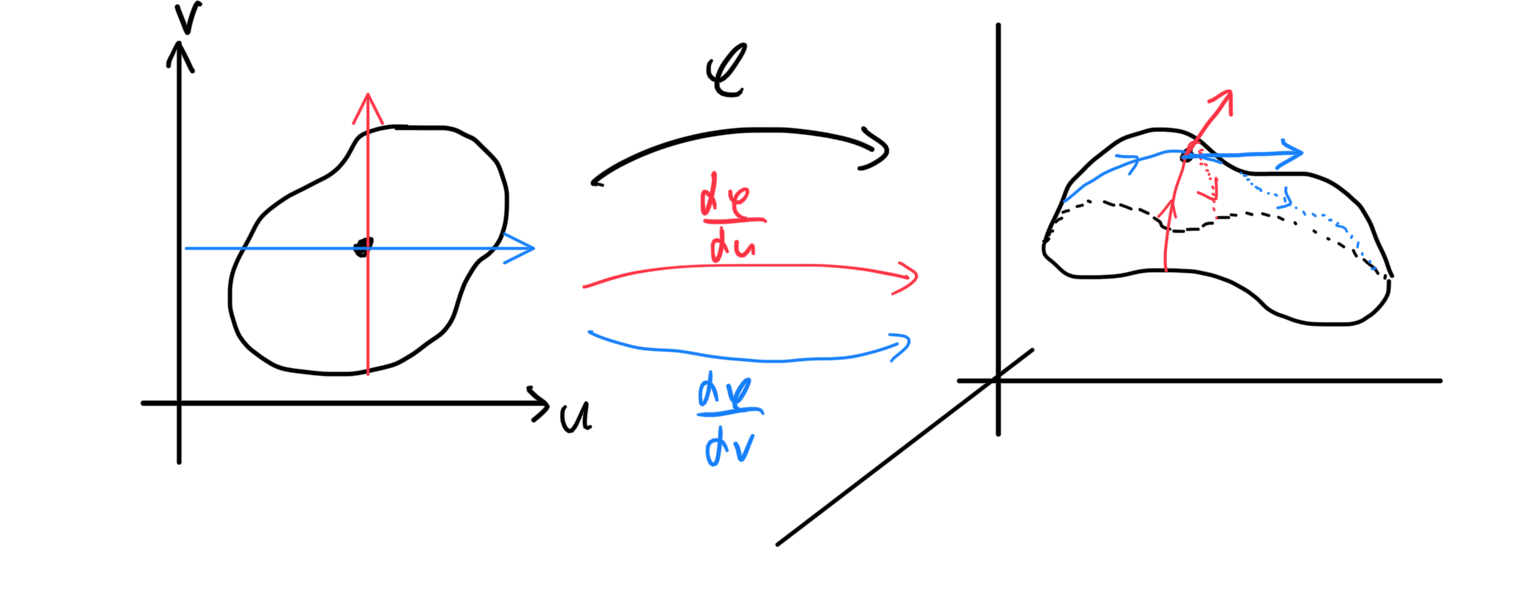
\includegraphics[scale=0.28]{img/Partial_Derivatives_with_respect_to_U_V.PNG}
		\caption{When $\varphi: D \subset \mathbb{R}^2 \to \mathbb{R}^3$, we can see visually that given $(u_0, v_0) \in D$, there should be two linearly independent tangent vectors $T_u, T_v$ sticking out from $\varphi(u_0, v_0)$ on the surface $E$. So every vector in the ``tangent plane'' should be a linear combination of $T_u$ and $T_v$. In fact, these two vectors are precisely $T_u = \frac{\partial \varphi}{\partial u} (u_0, v_0)$ and $T_v = \frac{\partial \varphi}{\partial v} (u_0, v_0)$, so the tangent plane is really just $\varphi(u_0, v_0)$ plus the vectors in the column space of $D \varphi(u_0, v_0)$!}
		\label{fig:Partial_Derivatives_with_respect_to_U_V}
	\end{figure}

	\begin{definition}[Tangent Space]
		Let $\varphi: D \subset \mathbb{R}^k \to \mathbb{R}^n$ be a regular parameterization, and let $u \in D$ be an interior point. The \textbf{tangent space} to the parameterized set at $\varphi(u)$ is the $k$-dimensional subspace
		\begin{equation}
			T_{\varphi(u)}E \coloneqq \operatorname{Im} D\varphi_u \subset \mathbb{R}^n.
		\end{equation}
		The corresponding \textbf{affine tangent plane} is
		\begin{equation}
			\varphi(u) + T_{\varphi(u)}E = \{ \varphi(u) + v : v \in T_{\varphi(u)}E \}.
		\end{equation}
	\end{definition}

	If $k=n-1$, then the normal space is one-dimensional. If $N(u)$ is a nonzero vector satisfying $N(u) \perp T_{\varphi(u)}E$, then the affine tangent hyperplane can also be written as
	\begin{equation}
		\{x \in \mathbb{R}^n : \langle x - \varphi(u), N(u) \rangle = 0\}.
	\end{equation}

	Often, we work with $2$-parameterizations of some $E \subset\mathbb{R}^3$. Therefore, the definition for a regularity at a point $(u_1, u_2)$ is equivalent to 
	\begin{equation}
		\frac{\partial \varphi}{\partial u_1} (u_1, u_2) \times \frac{\partial \varphi}{\partial u_2} (u_1, u_2) \neq 0
	\end{equation}
	where $\times$ is the Euclidean cross product. 

	\begin{figure}[H]
		\centering 
		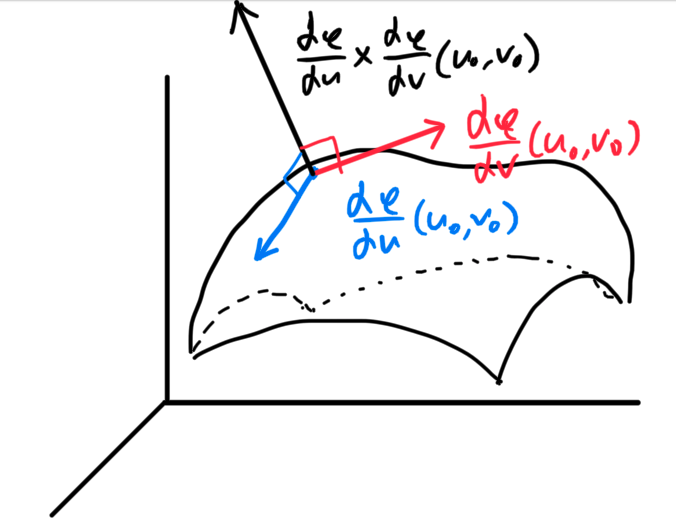
\includegraphics[scale=0.3]{img/Cross_Product_Regular_Surfaces.PNG}
		\caption{Note that the cross product $\frac{\partial \varphi}{\partial u} (u_0, v_0) \times \frac{\partial \varphi}{\partial v} (u_0, v_0) \neq 0$ if and only if $D\varphi (u_0, v_0)$ is full rank, i.e. the tangent plane exists.} 
		\label{fig:Cross_Product_Regular_Surfaces}
	\end{figure}

	A path has a natural orientation defined by the function. We would like to determine a similar notion of orientation by defining one ``side'' of a surface to be positive and the other to be negative. Surprisingly, a paramaterization does not have an intrinsic global orientation. Rather, we determine the orientation ourselves by choosing a unit vector that generally points towards the outside of the surface $S$. Again, this choice is arbitrary, but it is customary to choose a vector that generally points ``out.''

	\begin{definition}[Orientation of a Regular Parameterized Set]
		Let $\varphi : D \subset \mathbb{R}^k \to \mathbb{R}^n$ be a regular parameterization. The ordered tangent basis
		\begin{equation}
			D\varphi_p(e_1), \dots, D\varphi_p(e_k)
		\end{equation}
		determines an orientation of the tangent space
		\begin{equation}
			T_{\varphi(p)}E = \mathrm{Im}(D\varphi_p).
		\end{equation}
		An \textbf{orientation} of $E$ is a continuous choice of such positive tangent bases at each point of $E$.
	\end{definition}

  \begin{example}[Orientation of Surface]
		When $k=2$ and $n=3$, an orientation can equivalently be described by a continuous choice of unit normal vector
		\begin{equation}
			n(\varphi(u,v))
			=
			\pm
			\frac{\varphi_u(u,v)\times \varphi_v(u,v)}
			{\|\varphi_u(u,v)\times \varphi_v(u,v)\|}.
		\end{equation}

		\begin{figure}[H]
			\centering 
			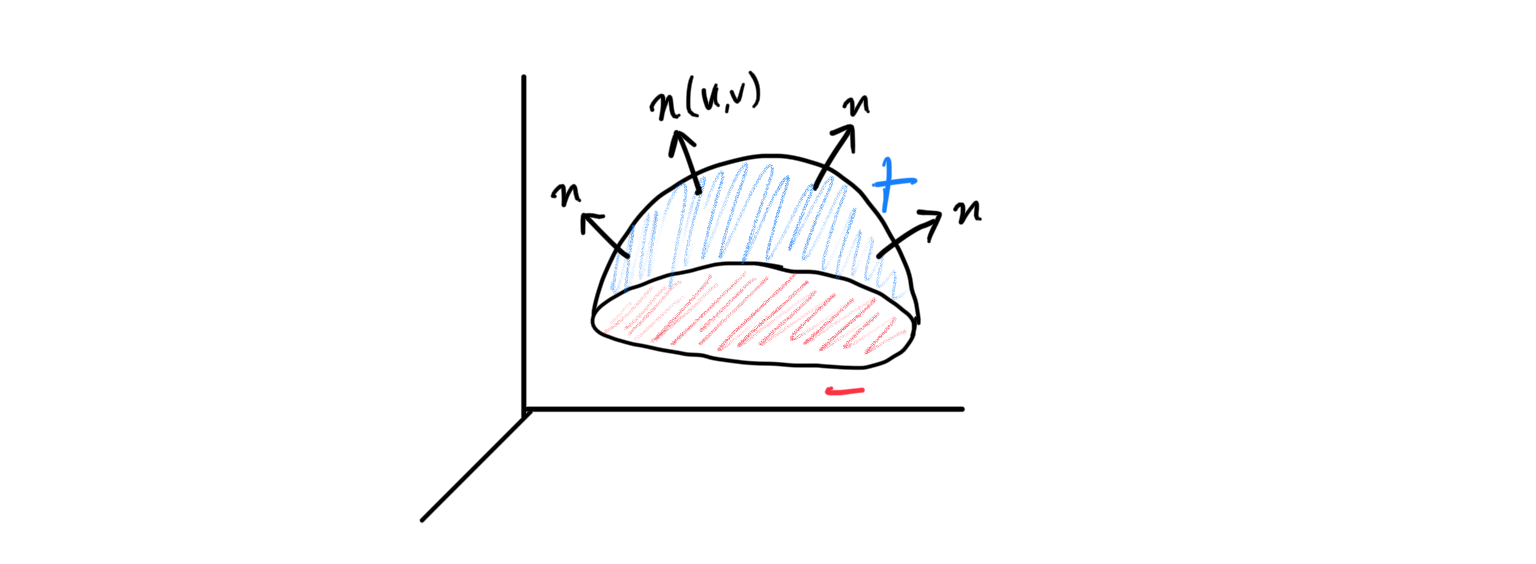
\includegraphics[scale=0.23]{img/Orientation_Unit_Vector.PNG}
			\caption{} 
			\label{fig:surface_orientation}
		\end{figure}
  \end{example}

	\begin{example}[Determining Orientation of an Ellipsoid]
		Consider the ellipsoid
		\begin{equation}
			E =
			\left\{
				(x,y,z) \in \mathbb{R}^3 :
				\frac{x^2}{a^2}
				+
				\frac{y^2}{b^2}
				+
				\frac{z^2}{c^2}
				=
				1
			\right\},
		\end{equation}
		where $a,b,c > 0$. A standard parameterization is
		\begin{equation}
			\varphi(u,v)
			=
			\big(
				a\sin u \cos v,
				b\sin u \sin v,
				c\cos u
			\big),
		\end{equation}
		where
		\begin{equation}
			0 \leq u \leq \pi,
			\qquad
			0 \leq v \leq 2\pi.
		\end{equation}
		The tangent vectors are
		\begin{equation}
			\varphi_u(u,v)
			=
			\big(
				a\cos u \cos v,
				b\cos u \sin v,
				-c\sin u
			\big)
		\end{equation}
		and
		\begin{equation}
			\varphi_v(u,v)
			=
			\big(
				-a\sin u \sin v,
				b\sin u \cos v,
				0
			\big).
		\end{equation}
		Their cross product is
		\begin{align}
			\varphi_u(u,v) \times \varphi_v(u,v)
			&=
			\big(
				bc\sin^2 u \cos v,
				ac\sin^2 u \sin v,
				ab\sin u \cos u
			\big).
		\end{align}

		To determine whether this points outward or inward, compare it with the
		position vector
		\begin{equation}
			\varphi(u,v)
			=
			\big(
				a\sin u \cos v,
				b\sin u \sin v,
				c\cos u
			\big).
		\end{equation}
		Compute the dot product:
		\begin{align}
			\left(\varphi_u \times \varphi_v\right) \cdot \varphi
			&=
			abc\sin^3 u \cos^2 v
			+
			abc\sin^3 u \sin^2 v
			+
			abc\sin u \cos^2 u \\
			&=
			abc\sin u
			\left(
				\sin^2 u \cos^2 v
				+
				\sin^2 u \sin^2 v
				+
				\cos^2 u
			\right) \\
			&=
			abc\sin u.
		\end{align}
		For $0<u<\pi$, we have $\sin u>0$, so
		\begin{equation}
			\left(\varphi_u \times \varphi_v\right) \cdot \varphi > 0.
		\end{equation}
		Hence $\varphi_u \times \varphi_v$ generally points away from the origin.
		Therefore, this parameterization induces the outward orientation on the
		ellipsoid.

		The corresponding unit normal vector field is
		\begin{equation}
			n(u,v)
			=
			\frac{\varphi_u(u,v) \times \varphi_v(u,v)}
			{\|\varphi_u(u,v) \times \varphi_v(u,v)\|}.
		\end{equation}
		If we wanted the inward orientation, we would use
		\begin{equation}
			-n(u,v)
			=
			-\frac{\varphi_u(u,v) \times \varphi_v(u,v)}
			{\|\varphi_u(u,v) \times \varphi_v(u,v)\|}.
		\end{equation}
	\end{example}

	\begin{example}[M\"obius Strip is Not Orientable]
		The M\"obius strip can be parameterized by
		\begin{equation}
			\varphi(u,v)
			=
			\bigg(
				\bigg(1 + \frac{v}{2}\cos\frac{u}{2}\bigg)\cos u,
				\bigg(1 + \frac{v}{2}\cos\frac{u}{2}\bigg)\sin u,
				\frac{v}{2}\sin\frac{u}{2}
			\bigg),
		\end{equation}
		where
		\begin{equation}
			0 \leq u \leq 2\pi,
			\qquad
			-1 \leq v \leq 1.
		\end{equation}
		Here $u$ moves around the central circle, while $v$ moves across the width
		of the strip. The factors $\cos(u/2)$ and $\sin(u/2)$ encode the half-twist.

		Notice that when $u = 0$,
		\begin{equation}
			\varphi(0,v)
			=
			\bigg(1+\frac{v}{2},0,0\bigg),
		\end{equation}
		while when $u = 2\pi$,
		\begin{equation}
			\varphi(2\pi,v)
			=
			\bigg(1-\frac{v}{2},0,0\bigg)
			=
			\varphi(0,-v).
		\end{equation}
		Thus, after going once around the strip, the transverse coordinate $v$ is
		reversed.

		This reversal is the geometric reason the M\"obius strip is not orientable.
		If we start with a normal vector $n$ at some point and move it continuously
		once around the strip, then after returning to the same point, the normal
		vector points in the opposite direction, namely $-n$. Therefore, there is no
		continuous way to choose a unit normal vector on the entire M\"obius strip.

		Hence the M\"obius strip is not orientable.
	\end{example}

\subsection{Line Integrals}

  \begin{definition}[Scalar Line Integral]
		Let $f: \mathbb{R}^n \to \mathbb{R}$, which can be interpreted as a scalar field. Now define a $C^1$ path function 
		\begin{equation}
			c: [a,b] \subset \mathbb{R} \to \mathbb{R}^n
		\end{equation}
		such that the composition of functions
		\begin{equation}
			f \circ c: [a, b] \subset \mathbb{R} \to \mathbb{R}^n
		\end{equation}
		is continuous. Then, the \textit{path integral}, or \textit{scalar line integral}, of $f$ along the path $c$. is defined
		\begin{align}
			\int_c f \;d s & = \int_a^b f\big(c(t)\big) ||c^\prime (t)|| \;d t \\
				& = \int_a^b f\big( x_1 (t), x_2 (t), ..., x_n (t)\big) ||c^\prime (t)|| \; d t
		\end{align}
		If $c(t)$ is only piece-wise $C^1$, we can define the path integral by breaking $[a,b]$ into pieces over with $f\big( c(t)\big) ||c^\prime (t)||$ is continuous and then summing the integrals over the pieces. 
		That is, 
		\begin{equation}
			\int_a^b f\big(c(t)\big) ||c^\prime (t)|| \;d t = \sum_{i = 0}^{n-1} \int_{\alpha_i}^{\alpha_{i+1}} f\big(c(t)\big) ||c^\prime (t)|| \; d t
		\end{equation}
  \end{definition}

  Note that since $f$ is a scalar-valued function, we can interpret a path integral as the sum of infinitesmal segments of the path $c$ having a weight determined by $f$ at each section. 
  If $f$ is a constant function outputting $1$ at every point, then the path integral just outputs the length of the path $c$ in $\mathbb{R}^n$. 
	\begin{equation}
  	L = \int_a^b f\big( c(t)\big) \|c^\prime (t)\| \, dt = \int_a^b \|c^\prime (t)\| \, d t
	\end{equation}

  \begin{definition}[Vector Line Integral]
		Let $F: \mathbb{R}^n \to \mathbb{R}^n$ be a vector field on $\mathbb{R}^n$ that is continuous on the $C^1$ oriented path $c: [a, b] \subset \mathbb{R} \to \mathbb{R}^n$. The \textit{line integral} of $F$ along $c$ is defined by the formula 
		\begin{equation}
			\int_c F \cdot d s = \int_a^b F\big( c(t)\big) \cdot c^\prime (t) \, d t
		\end{equation}
		where $\cdot$ represents the dot product of $F$ with $c^\prime$ over the interval $[a,b]$. It is also commonly written in differential notation, 
		\begin{equation}
			\int_c F \cdot ds = \int_c F \cdot (dx_1, \ldots, d x_n) = \int_c F_1 dx_1 + F_2 dx_2 + \ldots F_n dx_n
		\end{equation}

		\begin{figure}[H]
			\centering
			\begin{tikzpicture}[
				scale=1.2,
				% Define the style for placing exactly 12 red arrows evenly along the path
				path arrows/.style={
					postaction={decorate},
					decoration={
						markings,
						mark=between positions 0.05 and 0.98 step 0.085 with {\arrow[red, scale=1.2]{>}}
					}
				}
			]
				\begin{axis}[
					axis lines=center,
					view={0}{90}, % Locks the 3D axis into a top-down 2D view
					xmin=-3.2, xmax=3.2,
					ymin=-3.2, ymax=3.2,
					zmin=-1.0, zmax=1.0, % Fixes the empty axis range warning
					domain=-2.8:2.8,
					y domain=-2.8:2.8,
					samples=13, % Generates a 13x13 grid for the vector field
					ticks=none,
					clip=false
				]
					
					% The Vector Field: F(x,y) = <-y, x>
					% Opacity set to 0.2 to make it highly translucent/faded
					\addplot3[
						blue,
						opacity=0.2, 
						-stealth,
						quiver={
							u={-y},
							v={x},
							scale arrows=0.15,
							every arrow/.append style={line width=0.6pt}
						}
					] (x, y, 0);

					% The Oriented Path: A curved line from a to b
					\draw[thick, black, path arrows] 
						(-2.5, -1.5) .. controls (2.0, -2.5) and (-2.0, 2.5) .. (2.5, 1.5)
						node[pos=0, below left, black] {$a$}
						node[pos=1, above right, black] {$b$};

					% --- Specific Point P ---
					% Mathematically computed at t = 0.75 along the Bezier curve
					\coordinate (P) at (0.453, 1.312);
					
					% Draw Point P
					\fill[black] (P) circle (2pt) node[below right, xshift=2pt] {$P$};
					
					% Draw Tangent Vector T (Red)
					% True Direction at t=0.75 is <3.9375, 3.75>
					% Scaled down visually by ~0.3 for clarity -> <1.18, 1.12>
					\draw[red, -stealth, line width=1.5pt] 
						(P) -- ++(1.18, 1.12) node[right] {$\vec{T}$};

					% Draw Specific Field Vector F(P) (Blue, fully opaque)
					% True Field at P: F(0.453, 1.312) = <-1.312, 0.453>
					% Scaled up slightly for visual clarity -> <-0.787, 0.271>
					\draw[blue, -stealth, line width=1.5pt] 
						(P) -- ++(-0.787, 0.271) node[above left] {$\vec{F}(P)$};

				\end{axis}
			\end{tikzpicture}
			\caption{Visualizing a path integral. At a specific point $P$ along the oriented curve, the red tangent vector $\vec{T}$ points along the path, while the solid blue vector $\vec{F}(P)$ represents the local vector field at that exact location. The path integral $\int_C \vec{F} \cdot d\vec{r}$ accumulates the dot product of these two vectors at every point along the curve.}
			\label{fig:vector_field_tangent}
		\end{figure}
		
		Similarly with path integrals, we can also define line integrals as the sum of integrals over piece-wise continuous sections of $c$. That is, given an oriented curve $C$ made up of several oriented component curves $C_i$, $i = 1, 2, ..., k$, we can paramaterize $C$ by paramaterizing the pieces $C_i$'s separately. Thus, we can treat $C = C_1 + \ldots + C_k$ and get
		\begin{equation}
			\int_C F \cdot d s = \sum_{i = 1}^k \int_{C_i} F \cdot d s
		\end{equation}
		Note that a vector line integral is a generalization of scalar line integrals, so any results holding for vector line integrals also holds for their scalar counterpart. 
  \end{definition}

  \begin{example}[Work]
		In mechanics, \textbf{work} $W$ is defined as 
		\begin{equation}
			W = F \cdot d
		\end{equation}
		where $F$ is force and $d$ is displacement. With this knowledge, the reader can easily see that the work done by vector field $F$ on a particle traveling along a path $c$ from time $a$ to time $b$ can be calculated by the line integral
		\begin{align}
			W & = \int_a^b F\big( c(t)\big) \cdot c^\prime (t) \; d t \\
			& = \int_c F_1 dx + F_2 dy + F_3 dz
		\end{align}
  \end{example}

  \begin{theorem}[Invariance of Path Paramaterizations on Vector Line Integrals]
		Let $F$ be a vector field and $f$ be a scalar field, both continuous on the $C^1$ path function $p: [a,b] \to \mathbb{R}^n$ and let $q: [\alpha, \beta] \to \mathbb{R}^n$ be a reparamaterization of $p$. Then, 
		\begin{align*}
			q \text{ is orientation preserving} & \implies \int_p F \cdot d s = \int_q F \cdot d s \\
			q \text{ is orientation reversing} & \implies \int_p F \cdot d s = - \int_q F \cdot d s
		\end{align*}
  \end{theorem}
	
  We now introduce a fundamental theorem about line integrals over gradient fields. Recall the fundamental theorem of calculus. We can extend this to line integrals for functions mapping $\mathbb{R}^n$ to $\mathbb{R}$. 

  \begin{theorem}[Invariance of Line Integrals in Conservative Vector Fields]
		Given that $F: \mathbb{R}^n \to \mathbb{R}^n$ is a $C^1$ conservative vector field with $\nabla f = F$ for $C^2$ function $f: \mathbb{R}^n \to \mathbb{R}$ and path function $p: [a,b] \to \mathbb{R}^n$ is a piecewise $C^1$ path, then 
		\begin{equation}
			\int_p F \cdot d s = \int_p \nabla f \cdot d s = f\big(p(b)\big) - f\big(p(a)\big)
		\end{equation}
		That is, the line integral of any path in a conservative vector field is dependent on the value of $f$ at the endpoints $p(a)$ and $p(b)$. 

		\begin{figure}[H]
			\centering 
			\begin{tikzpicture}[
				scale=0.7,
				thick,
				black,
				% Define a style for adding an arrow to the middle of a path
				mid arrow/.style={
					postaction={decorate,
						decoration={markings,
							mark=at position #1 with {\arrow[scale=1.5]{>}}
						}
					}
				}
			]

				% 1. Define the start and end points
				\coordinate (A) at (0,0);
				\coordinate (B) at (8,1.5);

				% 2. Draw the points and their labels
				\fill (A) circle (2pt) node[below right, outer sep=3pt] {$p(a)$};
				\fill (B) circle (2pt) node[right, outer sep=2pt] {$p(b)$};

				% 3. Draw Path 1: Straight middle path
				\draw[mid arrow=0.5] (A) -- (B);

				% 4. Draw Path 2: Smooth upper path
				\draw[mid arrow=0.5] (A) to[bend left=30] (B);

				% 5. Draw Path 3: The highly convoluted upper outer path
				\draw[mid arrow=0.2, mid arrow=0.6, mid arrow=0.85] 
					(A) .. controls (-2, 2) and (0, 5) .. (3, 4)
							.. controls (6, 3) and (6, 6) .. (7.5, 3.5)
							.. controls (8, 2) and (9.5, 3.5) .. (B);

				% 6. Draw Path 4: The highly convoluted lower outer path
				\draw[mid arrow=0.1, mid arrow=0.35, mid arrow=0.6, mid arrow=0.85] 
					(A) .. controls (-2.5, -1) and (-1, -3) .. (0.5, -1.5)
							.. controls (2, 0) and (2.5, -4) .. (4, -2.5)
							.. controls (5.5, -1) and (5.5, -3) .. (7, -1.5)
							.. controls (8.5, 0) and (9, -1) .. (B);
			\end{tikzpicture}
			\caption{} 
			\label{fig:line_invariance}
		\end{figure} 
  \end{theorem}

  In physics, calculating the work done by a force represented by a vector field requires us to know the path that it travels through. 
	\begin{equation}
  	W = \int_p F \cdot ds
	\end{equation}
  However, in many cases $F$ is assumed to be conservative, so it is only necessary that we find the displacement of the particle from its endpoints, resulting in the simplification of the formula.  
	\begin{equation}
  	W = \int_p \nabla f \cdot ds = f\big( p(b)\big) - f \big(p(a)\big)
	\end{equation}

  \begin{corollary}[Equivalent Conditions for Vector Field to be Conservative]
		The following conditions are equivalent: 
		\begin{enumerate}
			\item $F: \mathbb{R}^n \to \mathbb{R}^n$ is a conservative vector field. 
			\item The line integral of $F: \mathbb{R}^n \to \mathbb{R}^n$ in curve $C$ is path independent; that is, if $C_1$ and $C_2$ are two paramaterizations of $C$, 
			\[\int_{C_1} F \cdot ds = \int_{C_2} F \cdot ds\]
			\item Given that $C$ is a closed loop, the line integral of $F: \mathbb{R}^n \to \mathbb{R}^n$ across $C$ is $0$. 
			\[\oint_C F \cdot ds = 0\]
			\item The curl of $F: \mathbb{R}^3 \to \mathbb{R}^3$ vanishes
			\[\curl{F} = \nabla \times F = \begin{pmatrix}
			\frac{\partial F}{\partial x} \\\frac{\partial F}{\partial y} \\\frac{\partial F}{\partial z} 
			\end{pmatrix} \times \begin{pmatrix}
			F_1\\F_2\\F_3
			\end{pmatrix}= 0\]
			\item The following partial derivatives of $F: \mathbb{R}^2 \to \mathbb{R}^2$ are equal
			\[\frac{\partial F_1}{\partial y} = \frac{\partial F_2}{\partial x}\]
		\end{enumerate}
  \end{corollary}

  We can develop a bit of intuition to determine whether a vector field is conservative or not. If vector field $F$ is conservative, then there exists a smooth scalar field $f$ such that $\nabla f = F$. For each latitude and longitude on a certain map, we can give it an altitude as a function of those coordinates (picture a map with a bunch of hills and valleys). The gradient and thus the vector field is all the vectors that point in the direction of highest ascent. he vector field is all the vectors that point in the direction of highest ascent. Extending the metaphor the path integral is like starting on at a point and climbing the hills and valleys, creating work as you go up a hill (proportional to the steepness and thus the dot product of your motion vector with the gradient vector field in the path integral) and decreasing the work you put in by going down a hill. Since the path is closed, it is like you are going up and down the same amount overall, so the path integral is zero. Following this analogy, the vector field determined by this function (marked as arrows in the $x, y$ plane) is conservative. 

	\begin{figure}[H]
		\centering
		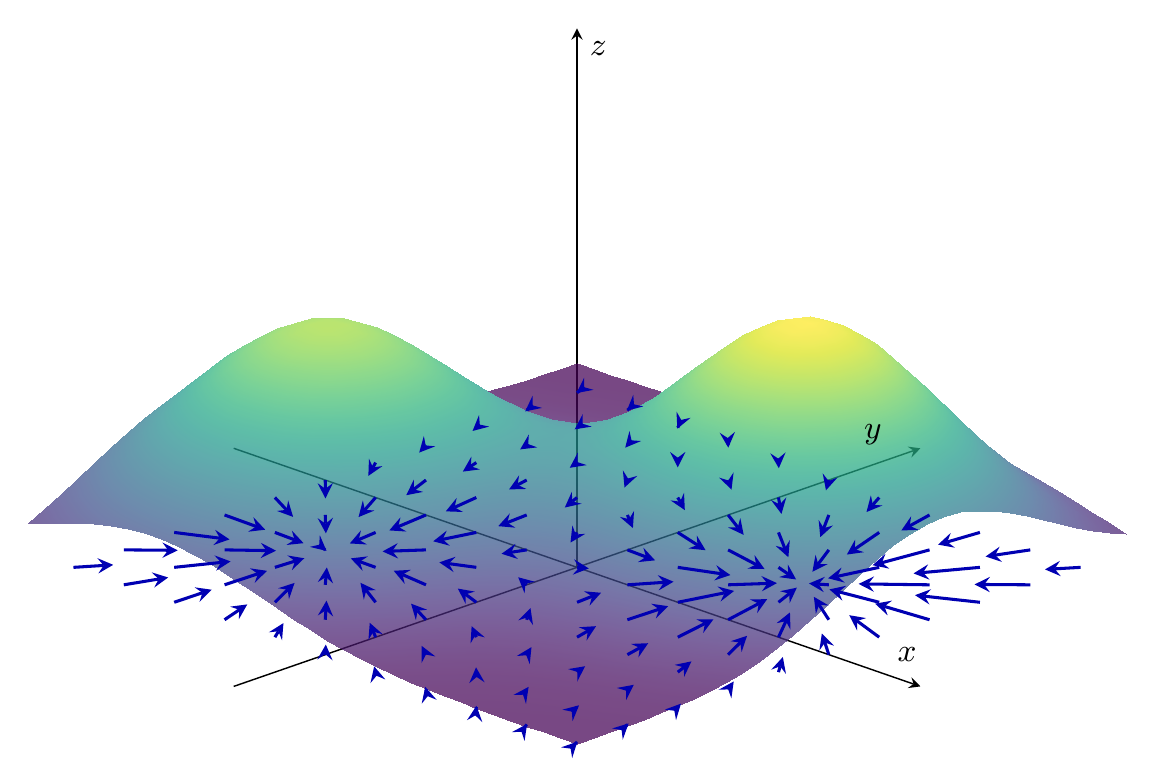
\begin{tikzpicture}[scale=1.3]
			\begin{axis}[
				view={45}{32},
				axis lines=center,
				xlabel={$x$},
				ylabel={$y$},
				zlabel={$z$},
				xmin=-3, xmax=3,
				ymin=-3, ymax=3,
				zmin=0, zmax=4.8,
				domain=-2.4:2.4,
				y domain=-2.4:2.4,
				samples=34,
				samples y=34,
				width=15cm,
				height=11.5cm,
				grid=major,
				ticks=none,
				tick label style={font=\small},
				label style={font=\small},
				colormap/viridis,
				clip=false
			]
				\addplot3[
					surf,
					opacity=0.72,
					shader=interp,
					draw=black!20
				]
				{2.2*exp(-((x-1.2)^2 + (y-0.8)^2)/1.6)
				+ 1.9*exp(-((x+1.3)^2 + (y+0.9)^2)/1.8)
				+ 0.12};

				\addplot3[
					blue!70!black,
					-stealth,
					samples=11,
					samples y=11,
					domain=-2.2:2.2,
					y domain=-2.2:2.2,
					quiver={
						u={-2.75*(x-1.2)*exp(-((x-1.2)^2 + (y-0.8)^2)/1.6)
							-2.11*(x+1.3)*exp(-((x+1.3)^2 + (y+0.9)^2)/1.8)},
						v={-2.75*(y-0.8)*exp(-((x-1.2)^2 + (y-0.8)^2)/1.6)
							-2.11*(y+0.9)*exp(-((x+1.3)^2 + (y+0.9)^2)/1.8)},
						w={0},
						scale arrows=0.3,
						every arrow/.append style={line width=0.85pt}
					}
				]
				(x,y,0);
			\end{axis}
		\end{tikzpicture}
		\caption{The vector field on the $xy$-plane is a conservative vector field since it is the gradient of the scalar field $f(x,y)=2.2e^{-((x-1.2)^2+(y-0.8)^2)/1.6}+1.9e^{-((x+1.3)^2+(y+0.9)^2)/1.8}+0.12$. The arrows on the $xy$-plane point in the direction of steepest ascent on the surface.}
		\label{fig:conservative_gradient_surface}
	\end{figure}

  If we can construct a closed loop around $F$ where the line integral is nonzero, then it means that we have ended up at a "higher" or "lower" (altitude) at the same point. This means that rather than being a certain landscape, there exist different "levels" of values at one point, like a spiraling staircase. For example, look at the solenoidal vector field below, where we can construct a closed loop (a circle going around the origin counterclockwise). There is no "surface" that can be defined such that it contains the solenoid. 

	\begin{figure}[H]
		\centering 
		\begin{tikzpicture}[
				scale=1.5,
				% Define the 3D perspective projection
				x={(-0.6cm, -0.4cm)}, 
				y={(1cm, 0cm)}, 
				z={(0cm, 1cm)},
				% Style for the black orthogonal axes
				axis/.style={thick, black, line cap=round},
				% Style for the blue solenoidal path and its arrows
				solenoid/.style={
					line width=1.5pt,
					postaction={
						decorate,
						decoration={
							markings,
							% Place intermediate arrows evenly along the path
							mark=between positions 0.03 and 0.95 step 0.055 with {
								\arrow[thick, scale=1.2]{>}
							},
							% Place the final larger arrow at the very end of the path
							mark=at position 1 with {
								\arrow[thick, scale=1.8]{>}
							}
						}
					}
				}
			]
				% 1. Draw 3D Axes
				\draw[axis] (0,0,0) -- (0,0,6.5);   % Z-axis (pointing up)
				\draw[axis] (0,0,0) -- (0,5.5,0);   % Y-axis (pointing right)
				\draw[axis] (0,0,0) -- (5.5,0,0);   % X-axis (pointing forward/left)

				% 2. Draw the starting point dot
				% Evaluated at t=0 for the parametric equations below
				\fill ({2*cos(0) + 2}, {2*sin(0) + 2}, 0) circle (2pt);

				% 3. Plot the Solenoidal Path
				% Using a parametric math engine (t represents degrees by default)
				\draw[
					solenoid,
					variable=\t, 
					domain=0:1850, % 5 full coils + a slight continuation
					samples=100,   % High sample rate ensures a perfectly smooth curve
					smooth
				] 
				plot ({2*cos(\t) + 2}, {2*sin(\t) + 2}, {\t/300});
		\end{tikzpicture}
		\caption{} 
		\label{fig:solenoid_nonconservative}
	\end{figure}

  Clearly, as a particle travels through the vector field along the path, it does positive work while it has zero displacement, and clearly, there exists no function that can output both these values as determined by vector field $F$. 

  \begin{theorem}[Helmholtz Decomposition]
		Let $F: \mathbb{R}^3 \to \mathbb{R}^3$ be a $C^2$ vector field. Then, $F$ can be decomposed into a curl-free component and a divergence-free component. That is, there exists vector fields $A$ and $\Phi$
		\begin{equation}
			F = - \nabla \cdot \Phi + \nabla \times A
		\end{equation}
  \end{theorem}


  \begin{definition}[Curvature at a Point]
		Let $c: [a, b] \to C \subset \mathbb{R}^3$ be a unit-speed paramaterization of $C$, meaning that $||c^\prime (t)|| = 1$ for all $t \in [a,b]$, and let $p = c(t_0)$ be a point in $C$. The \textit{curvature} $\kappa(p)$ at $p$ is a mapping defined
		\begin{equation}
			\kappa: C \to \mathbb{R}, \;\; \kappa(p) \coloneqq ||c^{\prime \prime} (t_0)||
		\end{equation}
		Notice that since we require a unit speed paramaterization of $C$, we do not need to worry about how a given curve is paramaterized. 
  \end{definition}

  Since the curvature is defined pointwise for each point in curve $C$, we can integrate over all the curvatures in $C$ to define the total curvature. 

  \begin{definition}[Total Curvature]
		The \textit{total curvature} of a curve $c: [a,b] \to C \subset \mathbb{R}^3$ is the scalar line integral 
		\begin{equation}
			\int_C \kappa \, ds
		\end{equation}
  \end{definition}

  \begin{theorem}[Fary-Milnor Theorem]
		Given a unit speed paramaterization $c: [a,b] \to C \subset \mathbb{R}^3$, if $C$ is closed (that is, $c(a)=c(b)$), then 
		\begin{equation}
			\oint_C \kappa\, ds \geq 2 \pi
		\end{equation}
		and equals $2\pi$ only when $C$ is a circle. Furthermore, if $C$ is a closed space curve with 
		\begin{equation}
			\oint_C \kappa\, ds \leq 4\pi
		\end{equation}
		then $C$ is "unknotted." That is, $C$ can be continuously deformed without every intersecting itself into a planar circle. Therefore, for knotted curves $C$, we have
		\begin{equation}
			\oint_C \kappa \, ds > 4\pi
		\end{equation}
  \end{theorem}

\subsection{Surface Integrals}

  Surface integrals are the $2$-dimensional analogue, or the double integral version, of line integrals. It is the integration of surfaces. A physical interpretation of a scalar surface integral is the weighted surface area of a certain surface. 

  \begin{definition}[Scalar Surface Integrals]
		Let $f: \mathbb{R}^3 \to \mathbb{R}$ be a $C^1$ scalar field defined on a paramaterized surface $S \subset \mathbb{R}^3$ with paramaterization $\varphi: D \subset \mathbb{R}^2 \to \mathbb{R}^3$. That is, $\varphi(D) = S$. We define the integral $f$ over $S$ to be
		\begin{align}
			\iint_S f \; dS & = \iint_S f(x, y, z) \; dS \\
			& = \iint_D f\big( \varphi(u, v)\big) \bigg|\bigg|\frac{\partial \varphi}{\partial u} \times \frac{\partial \varphi}{\partial v}\bigg|\bigg| \; du \,dv
		\end{align}
		Note that this will require us to transform $f$, a function of $x, y, z$, into the function $f \circ \varphi$ of $u, v$. Additionally, if the paramaterization of the surface $S$ is not defined, then it one must be constructed. It is also clear that if $S$ is a union of surfaces $S_i$, then its surface integral is the sum of the surface integrals of the $S_i$'s. 
  \end{definition}

  Letting the scalar field $f$ be the constant field equal to $1$, the scalar surface integral measures the surface area of $S$. 
  \[A(S) = \iint_S \; dS = \iint_D \Big|\Big|\frac{\partial \varphi}{\partial u} \times \frac{\partial \varphi}{\partial v}\Big|\Big| \; du\, dv\]
  It is easy to see that the orientation of the paramaterization $\varphi$ does not affect scalar surface integrals, since the sign of the orientation gets nullified by the absolute value sign over $||\frac{\partial \varphi}{\partial u} \times \frac{\partial \varphi}{\partial v}||$. 

  Its physical interpretation is to measure the rate at which a fluid (determined by a vector field $F$) is crossing a given surface $S$. It also has many applications in electromagnetism. 

  \begin{definition}[Vector Surface Integrals]
		Let $F$ be a vector field defined on surface $S$, the image of a paramaterized surface $\varphi$. The \textit{surface integral} of $F$ over $S$ is defined below, which is equivalent to summing up the dot product of the vector field and the normal vector to the surface. 
		\begin{center}
			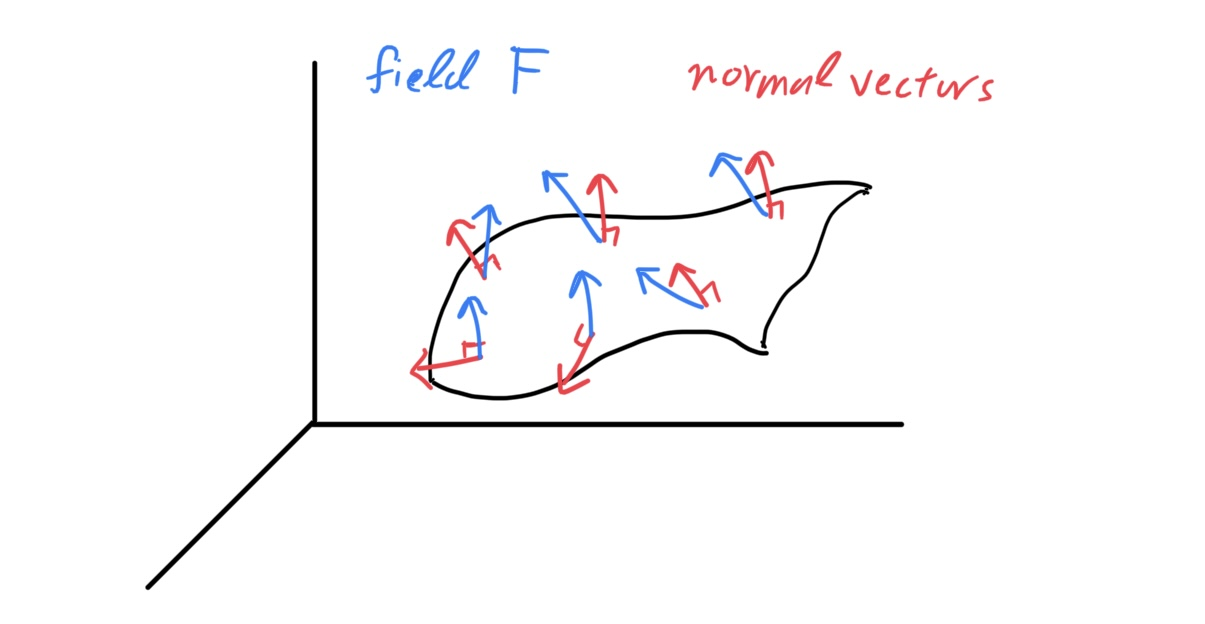
\includegraphics[scale=0.3]{img/Vector_Surface_Integral.jpg}
		\end{center}
		It can be calculated with the following formulas by converting it into a scalar surface integral where the scalar field is the value of the dot product of the vector field with the normal vectors of the surface. 
		\begin{align}
			\iint_{S} F \cdot d S & = \iint_S (F \cdot n) \; dS \\
			& = \iint_D \Bigg( F\big( \varphi(u, v)\big) \cdot \frac{\frac{\partial \varphi}{\partial u} \times \frac{\partial \varphi}{\partial v}}{\Big|\Big|\frac{\partial \varphi}{\partial u} \times \frac{\partial \varphi}{\partial v} \Big|\Big|} \Bigg) \, \bigg|\bigg|\frac{\partial \varphi}{\partial u} \times \frac{\partial \varphi}{\partial v}\bigg|\bigg|\; du\,dv \\
			& = \iint_D F\big(\varphi(u, v)\big) \cdot \bigg( \frac{\partial \varphi}{\partial u} \times \frac{\partial \varphi}{\partial v}\bigg) \; du\,dv
		\end{align}
  \end{definition}

  Since we are now talking about vector fields, the orientation of the paramaterization is now significant. Visually, if the orientation of the surface $S$ generally aligns with the vector field $F$, then the integral will be positive (since two vectors $\alpha, \beta$ generally pointing in the same direction implies that $\alpha \cdot \beta > 0$). The orientation of the paramaterization, which is dependent on $\frac{\partial \varphi}{\partial u} \times \frac{\partial \varphi}{\partial v}$, determines the direction of the normal vector $n$ (since it is defined to be $(\frac{\partial \varphi}{\partial u} \times \frac{\partial \varphi}{\partial v}) / \big|\big|\frac{\partial \varphi}{\partial u} \times \frac{\partial \varphi}{\partial v}\big|\big|$. Therefore, changing the orientation of $\varphi$ will reverse the direction of $n$, which will then reverse the sign of the integral since $n$ now points in the opposite direction of the vector field $F$ than it previously did (by reversing the sign of the dot products). This is formalized in the theorem below. 

  \begin{theorem}[Invariance Vector Surface Integrals Under Parameterization]
		Let $S$ be an oriented surface and let $\varphi_1$ and $\varphi_2$ be two regular paramaterizations with $F$ a continuous vector field defined on $S$. Then, assuming $\varphi_1$ is orientation preserving, 
		\begin{align}
			\varphi_2 \text{ is orientation preserving } & \implies \iint_{\varphi_1} F \cdot d S = \iint_{\varphi_2} F \cdot d S \\
			\varphi_2 \text{ is orientation reversing } & \implies - \iint_{\varphi_1} F \cdot d S = \iint_{\varphi_2} F \cdot d S 
		\end{align}
  \end{theorem}

	\begin{theorem}[Surface Integral Formula for Graphs]
		Given that we have the graph of a function $g: \mathbb{R}^2 \to \mathbb{R}$ rather than a general surface, we can paramaterize it simply as
		\begin{equation}
			\varphi(u, v) \coloneqq \big(u, v, g(u, v) \big)
		\end{equation}

		This means that 
		\begin{equation}
			\frac{\partial \varphi}{\partial u} \times \frac{\partial \varphi}{\partial v} = 
			\begin{pmatrix}
			-\frac{\partial g}{\partial u} \\ -\frac{\partial g}{\partial v} \\ 1
			\end{pmatrix} \implies \bigg|\bigg|\frac{\partial \varphi}{\partial u} \times \frac{\partial \varphi}{\partial v} \bigg|\bigg| = \sqrt{1 + \Big(\frac{\partial g}{\partial u}\Big)^2 + \Big( \frac{\partial g}{\partial v}\Big)^2}
		\end{equation}

		So we can simplify the equation for the surface area $S$ of the graph of $g$ over the region $D$ in the $x y$-plane, as 
		\begin{align}
			A(S) & = \iint_S \; d S = \iint_D \bigg|\bigg|\frac{\partial \varphi}{\partial u} \times \frac{\partial \varphi}{\partial v} \bigg|\bigg| \; d A \\
			& = \iint_D \sqrt{1 + \Big(\frac{\partial g}{\partial u}\Big)^2 + \Big( \frac{\partial g}{\partial v}\Big)^2} \; d u \, d v
		\end{align}

		With the same $g$, we can find the weighed surface area of $S$ over the scalar function $f: \mathbb{R}^3 \to \mathbb{R}$ with the formula
		\begin{equation}
			\iint_S f \; d S = \iint_D f\big(u, v, g(u, v)\big) \sqrt{1 + \Big(\frac{\partial g}{\partial u}\Big)^2 + \Big( \frac{\partial g}{\partial v}\Big)^2} \; d u \, d v
		\end{equation}

		Finally, with the same graph $g$, the surface integral over the vector field $F$ is
		\begin{align}
			\iint_S F \cdot d S & = \iint_D F\big(\varphi(u, v)\big) \cdot \bigg( \frac{\partial \varphi}{\partial u} \times \frac{\partial \varphi}{\partial v}\bigg) \; d u \, d v \\
			& = \iint_D \bigg( F_1(u, v) \Big(- \frac{\partial g}{\partial u}\Big) + F_2 (u, v) \Big( - \frac{\partial g}{\partial v} \Big) + F_3 (u, v) \bigg) \; d u \, d v
		\end{align}
	\end{theorem}

\subsection{Green Theorem}

  Recall the differential notation for writing line integrals. For 2 and 3 dimensions, it is written as
  \begin{align}
		& \int_C F \cdot d s = \int_C F \cdot (d x, d y) = \int_C F_1 \, d x + F_2 \, d y \\
		& \int_C F \cdot d s = \int_C F \cdot (d x, d y, d z) = \int_C F_1 \, d x + F_2 \, d y + F_3 \, d z 
  \end{align}


  Green's Theorem gives the relationship between a line integral around a simple closed curve $C$ and a double integral over the plane region $D$ bounded by $C$. 

  \begin{theorem}[Green's Theorem in $\mathbb{R}^2$]
		Let there be a 2-dimensional $C^1$ vector field $F$ on $\mathbb{R}^2$ defined on a simple oriented closed piecewise-smooth curve $C$ and its bounded region $D \subset \mathbb{R}^2$ (that is, $C = \partial D$). Let the orientation of the path of $C$ be such that it is traveling \textit{counterclockwise}, i.e. a point traveling through $C$ would see the region $D$ to its \textit{left}, denoted as $C^+$ and the clockwise orientation as $C^-$.  Then, 
		\begin{equation}
			\oint_{C^+} F_1 \, d x + F_2 \, d y = \iint_D \bigg( \frac{\partial F_2}{\partial x} - \frac{\partial F_1}{\partial y} \bigg) \; d x \, d y
		\end{equation}
		By reversing the orientation, it is clear that we have
		\begin{equation}
			\oint_{C^-} F_1 \, d x + F_2 \, d y = - \iint_D \bigg( \frac{\partial F_2}{\partial x} - \frac{\partial F_1}{\partial y} \bigg) \; d x \, d y
		\end{equation}
		Note that this theorem is expressed in terms of the components of the vector field $F$. 
		\begin{center}
		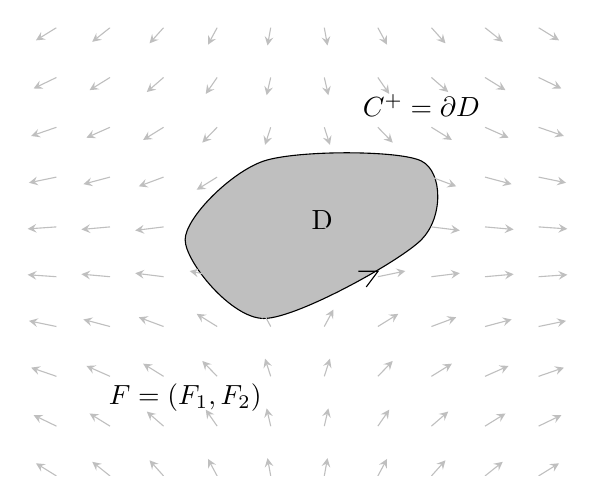
\begin{tikzpicture}
			\draw[fill=lightgray] plot [smooth cycle] coordinates {(2,3) (3,4) (5,4) (5,3) (3,2)};
			\node [above left] at (4,3) {D};
			\begin{axis}[view={0}{90}, hide axis, zmin=-1, zmax=1, tick label style={font=\tiny}]
			\addplot3 [lightgray,-stealth,samples=10,
					quiver={
							u={3*x/pow(x^2 + y^2,1/2)},
							v={-2*y/pow(x^2 + y^2,1/2)},
							scale arrows=0.2,
					},] {0};
			\end{axis}
			\node at (2,1) {$F = (F_1, F_2)$};
			\node at (5,4.7) {$C^+ = \partial D$};
			\draw (4.3,2.4)--(4.45,2.6)--(4.2,2.6);
		\end{tikzpicture}
		\end{center}
  \end{theorem}

  Green's theorem has many applications in physics. For example, in order to solve two-dimensional flow integrals measuring the sum of fluid outflowing from a volume, Green's theorem allows us to calculate the total outflow summed about an enclosing area . 

  \begin{corollary}
		Let $D$ be a region for which Green's theorem applies with positively oriented boundary $\partial D$. Then, the area of $D$ can be computed with the formula
		\begin{equation}
			A(D) = \frac{1}{2} \oint_{\partial D} x \, d y - y \, d x
		\end{equation}
  \end{corollary}

  Green's theorem can be used to determine the area of centroid of plane figures solely by integrating over the perimeter. 

\subsection{Stokes' Theorem}

  Green's theorem relates line integrals to double integrals. Stokes' theorem generalizes Green's theorem by relating line integrals to surface integrals of 2-dimensional surfaces embedded in $\mathbb{R}^3$. 

  \begin{theorem}[Stokes' Theorem]
		Let $S$ be an oriented regular surface defined by paramaterization $\varphi: D \subset \mathbb{R}^2 \to \mathbb{R}^3$, and let the image of the boundary $\partial D$ under $\varphi$ be the boundary $\partial S$ of $S$. 

		\begin{figure}[H]
			\centering
			\begin{tikzpicture}
				\begin{axis}[
					view={125}{22},
					axis lines=center,
					xmin=-0.2, xmax=5.6,
					ymin=-0.2, ymax=6.6,
					zmin=0, zmax=2.4,
					ticks=none,
					width=9cm,
					height=7cm,
					colormap/viridis,
					clip=false,
					disabledatascaling % Disables the massive internal scaling causing the crash
				]
					\addplot3[
						surf,
						domain=0:360,
						y domain=0:1,
						variable=u,        % Removed backslash
						variable y=r,      % Removed backslash
						samples=18,
						samples y=5,
						point meta=z,
						mesh,
						draw=black!45,
						shader=flat
					]
					({4 + 1.9*r*cos(u)}, {6.6 + 2.35*r*sin(u)}, {2.55 - 0.45*r^2});

					\addplot3[
						blue!70!black,
						line width=0.9pt,
						domain=35:395,
						variable=u,        % Removed backslash
						samples=40,
						postaction={decorate},
						decoration={
							markings,
							mark=between positions 0.125 and 0.875 step 0.05 with {\arrow[scale=1.5]{stealth}}
						}
					]
					({4 + 1.9*cos(u)}, {6.6 + 2.35*sin(u)}, {2.10});

					\addplot3[thick, -stealth]
					coordinates {(4,6.6,2.55) (4,6.6,3.25)};

					\node at (axis cs:4.95,7.45,2.58) {$S$};
					\node[blue!70!black] at (axis cs:5.15,5.05,2.08) {$\partial S$};
					\node[right] at (axis cs:4,6.6,3.28) {$n$};
				\end{axis}
			\end{tikzpicture}
			\caption{The orientation unit vector $n$ of $S$ induces the positive orientation of $\partial S$, denoted $\partial S^+$. Visually, if you are walking along the curve with your head is pointing in the same direction as the unit normal vectors while the surface is on the left then you are walking in the positive direction on $\partial S$. }
		\end{figure}

		Given that $F$ is a $C^1$ vector field defined on $S$, then
		\begin{equation}
			\iint_S \curl{F} \cdot dS = \iint_S \big( \nabla \times F \big) \cdot d S = \oint_{\partial S^+} F \cdot d s
		\end{equation}
		If $S$ has no boundary, that is, if the image of $p^\prime = \partial S$ is not a simple closed curve, then the integral is $0$. 
  \end{theorem}

  The above theorem implies that the vector surface integral of a surface without a boundary (i.e. a closed graph, such as a sphere) is always $0$ along the curl of any $C^1$ field. Geometrically, this means that given a closed solid $S$ with field $\nabla \times F$, the rate of flow of the vector field into $S$ is equal to the flow out of $S$. 

\subsection{Gauss' Theorem}

  The divergence theorem relates the flux of a vector field through a closed surface to the divergence of the field in the volume enclosed. 

  \begin{theorem}[Gauss' Divergence Theorem]
		Let $V$ be a subset of $\mathbb{R}^3$. Denote by $\partial V$ the oriented closed surface that bounds $V$ (with outward pointing normal orientation vectors), and let $F$ be a $C^1$ vector field defined on a neighborhood of $V$. Then, 
		\begin{equation}
			\iiint_V \Div{F} \, d V = \iiint_V (\nabla \cdot F) \, d V = \oiint_{\partial V} F \cdot d S = \oiint_{\partial V} (F \cdot n) \, dS
		\end{equation}
		where the two left-most integrals are volume integrals, and the two right-most integrals are surface integrals. 

		\begin{figure}[H]
			\centering 
			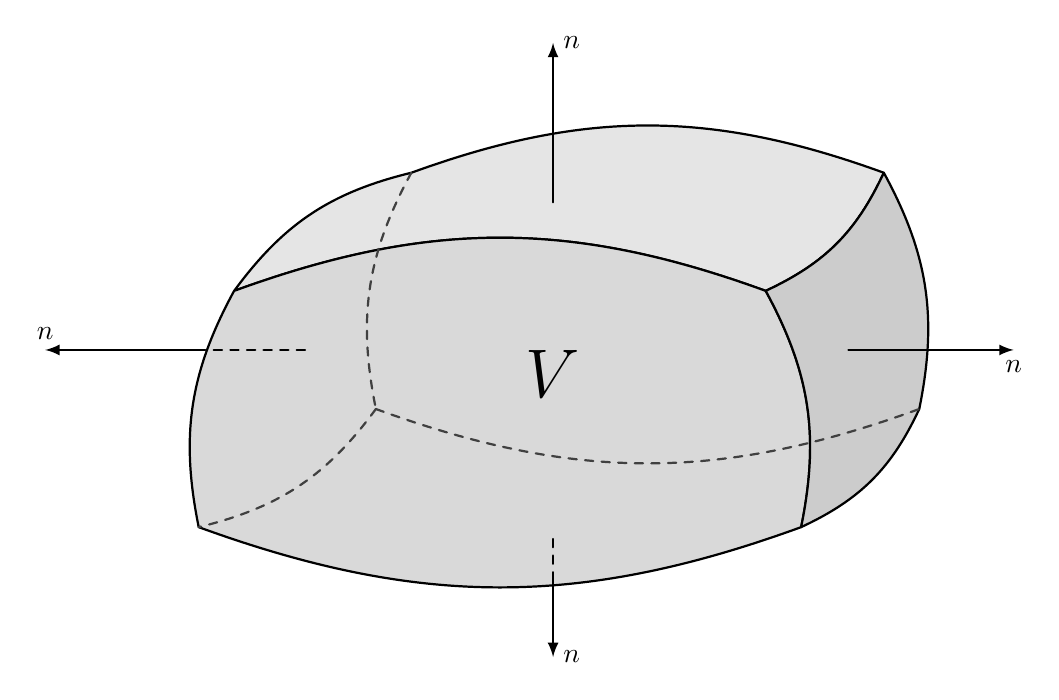
\begin{tikzpicture}[
					scale=1.5,
					line join=round,
					line cap=round
				]
					% 1. Coordinates for the 8 corners of the blob
					\coordinate (FL) at (-2.5, 0.5);   % Front Top Left
					\coordinate (FR) at (2.0, 0.5);    % Front Top Right
					\coordinate (FBL) at (-2.8, -1.5); % Front Bottom Left
					\coordinate (FBR) at (2.3, -1.5);  % Front Bottom Right
					
					\coordinate (TL) at (-1.0, 1.5);   % Back Top Left
					\coordinate (TR) at (3.0, 1.5);    % Back Top Right
					\coordinate (BBL) at (-1.3, -0.5); % Back Bottom Left
					\coordinate (BBR) at (3.3, -0.5);  % Back Bottom Right

					% 2. Fill visible faces with flat shades of gray
					% Top face
					\filldraw[fill=gray!20, draw=black, thick] 
						(TL) to[bend left=20] (TR) 
						to[bend left=20] (FR) 
						to[bend right=20] (FL) 
						to[bend left=20] cycle;
						
					% Front face
					\filldraw[fill=gray!30, draw=black, thick] 
						(FL) to[bend left=20] (FR) 
						to[bend left=20] (FBR) 
						to[bend left=20] (FBL) 
						to[bend left=20] cycle;
						
					% Right face
					\filldraw[fill=gray!40, draw=black, thick] 
						(FR) to[bend right=20] (TR) 
						to[bend left=20] (BBR) 
						to[bend left=20] (FBR) 
						to[bend right=20] cycle;

					% 3. Draw dashed hidden lines (back and bottom edges)
					\draw[dashed, darkgray, thick] (TL) to[bend right=20] (BBL);
					\draw[dashed, darkgray, thick] (BBL) to[bend left=20] (FBL);
					\draw[dashed, darkgray, thick] (BBL) to[bend right=20] (BBR);

					% 4. Draw Normal Vectors (Orthogonal to the viewing plane)
					\tikzset{normal vector/.style={-latex, thick, black}}
					
					% Top normal
					\draw[normal vector] (0.2, 1.25) -- (0.2, 2.6) node[right] {$\boldsymbol{n}$};
					
					% Bottom normal (partially hidden inside the volume)
					\draw[dashed, thick] (0.2, -1.6) -- (0.2, -1.9);
					\draw[normal vector] (0.2, -1.9) -- (0.2, -2.6) node[right] {$\boldsymbol{n}$};
					
					% Left normal (partially hidden inside the volume)
					\draw[dashed, thick] (-1.9, 0) -- (-2.8, 0);
					\draw[normal vector] (-2.8, 0) -- (-4.1, 0) node[above] {$\boldsymbol{n}$};
					
					% Right normal (starts on the right face surface)
					\draw[normal vector] (2.7, 0) -- (4.1, 0) node[below] {$\boldsymbol{n}$};

					% 5. Center Volume Label 'V'
					\node at (0.2, -0.2) {\Huge $V$};
			\end{tikzpicture}
			\caption{} 
			\label{fig:gauss_theorem}
		\end{figure}
  \end{theorem}

	Intuitively, this makes sense; the volume integrals represent the total of the sources in volume $V$, and the right hand side represents the total flow across the boundary $\partial V$. 
